\documentclass[ignorenonframetext,]{beamer}
\setbeamertemplate{caption}[numbered]
\setbeamertemplate{caption label separator}{: }
\setbeamercolor{caption name}{fg=normal text.fg}
\beamertemplatenavigationsymbolsempty
\usepackage{lmodern}
\usepackage{amssymb,amsmath}
\usepackage{ifxetex,ifluatex}
\usepackage{fixltx2e} % provides \textsubscript
\ifnum 0\ifxetex 1\fi\ifluatex 1\fi=0 % if pdftex
  \usepackage[T1]{fontenc}
  \usepackage[utf8]{inputenc}
\else % if luatex or xelatex
  \ifxetex
    \usepackage{mathspec}
  \else
    \usepackage{fontspec}
  \fi
  \defaultfontfeatures{Ligatures=TeX,Scale=MatchLowercase}
\fi
% use upquote if available, for straight quotes in verbatim environments
\IfFileExists{upquote.sty}{\usepackage{upquote}}{}
% use microtype if available
\IfFileExists{microtype.sty}{%
\usepackage{microtype}
\UseMicrotypeSet[protrusion]{basicmath} % disable protrusion for tt fonts
}{}
\newif\ifbibliography
\hypersetup{
            pdftitle={Introduction to statistics and probability},
            pdfauthor={Leanne Dong},
            pdfborder={0 0 0},
            breaklinks=true}
\urlstyle{same}  % don't use monospace font for urls
\usepackage{color}
\usepackage{fancyvrb}
\newcommand{\VerbBar}{|}
\newcommand{\VERB}{\Verb[commandchars=\\\{\}]}
\DefineVerbatimEnvironment{Highlighting}{Verbatim}{commandchars=\\\{\}}
% Add ',fontsize=\small' for more characters per line
\usepackage{framed}
\definecolor{shadecolor}{RGB}{248,248,248}
\newenvironment{Shaded}{\begin{snugshade}}{\end{snugshade}}
\newcommand{\KeywordTok}[1]{\textcolor[rgb]{0.13,0.29,0.53}{\textbf{#1}}}
\newcommand{\DataTypeTok}[1]{\textcolor[rgb]{0.13,0.29,0.53}{#1}}
\newcommand{\DecValTok}[1]{\textcolor[rgb]{0.00,0.00,0.81}{#1}}
\newcommand{\BaseNTok}[1]{\textcolor[rgb]{0.00,0.00,0.81}{#1}}
\newcommand{\FloatTok}[1]{\textcolor[rgb]{0.00,0.00,0.81}{#1}}
\newcommand{\ConstantTok}[1]{\textcolor[rgb]{0.00,0.00,0.00}{#1}}
\newcommand{\CharTok}[1]{\textcolor[rgb]{0.31,0.60,0.02}{#1}}
\newcommand{\SpecialCharTok}[1]{\textcolor[rgb]{0.00,0.00,0.00}{#1}}
\newcommand{\StringTok}[1]{\textcolor[rgb]{0.31,0.60,0.02}{#1}}
\newcommand{\VerbatimStringTok}[1]{\textcolor[rgb]{0.31,0.60,0.02}{#1}}
\newcommand{\SpecialStringTok}[1]{\textcolor[rgb]{0.31,0.60,0.02}{#1}}
\newcommand{\ImportTok}[1]{#1}
\newcommand{\CommentTok}[1]{\textcolor[rgb]{0.56,0.35,0.01}{\textit{#1}}}
\newcommand{\DocumentationTok}[1]{\textcolor[rgb]{0.56,0.35,0.01}{\textbf{\textit{#1}}}}
\newcommand{\AnnotationTok}[1]{\textcolor[rgb]{0.56,0.35,0.01}{\textbf{\textit{#1}}}}
\newcommand{\CommentVarTok}[1]{\textcolor[rgb]{0.56,0.35,0.01}{\textbf{\textit{#1}}}}
\newcommand{\OtherTok}[1]{\textcolor[rgb]{0.56,0.35,0.01}{#1}}
\newcommand{\FunctionTok}[1]{\textcolor[rgb]{0.00,0.00,0.00}{#1}}
\newcommand{\VariableTok}[1]{\textcolor[rgb]{0.00,0.00,0.00}{#1}}
\newcommand{\ControlFlowTok}[1]{\textcolor[rgb]{0.13,0.29,0.53}{\textbf{#1}}}
\newcommand{\OperatorTok}[1]{\textcolor[rgb]{0.81,0.36,0.00}{\textbf{#1}}}
\newcommand{\BuiltInTok}[1]{#1}
\newcommand{\ExtensionTok}[1]{#1}
\newcommand{\PreprocessorTok}[1]{\textcolor[rgb]{0.56,0.35,0.01}{\textit{#1}}}
\newcommand{\AttributeTok}[1]{\textcolor[rgb]{0.77,0.63,0.00}{#1}}
\newcommand{\RegionMarkerTok}[1]{#1}
\newcommand{\InformationTok}[1]{\textcolor[rgb]{0.56,0.35,0.01}{\textbf{\textit{#1}}}}
\newcommand{\WarningTok}[1]{\textcolor[rgb]{0.56,0.35,0.01}{\textbf{\textit{#1}}}}
\newcommand{\AlertTok}[1]{\textcolor[rgb]{0.94,0.16,0.16}{#1}}
\newcommand{\ErrorTok}[1]{\textcolor[rgb]{0.64,0.00,0.00}{\textbf{#1}}}
\newcommand{\NormalTok}[1]{#1}
\usepackage{graphicx,grffile}
\makeatletter
\def\maxwidth{\ifdim\Gin@nat@width>\linewidth\linewidth\else\Gin@nat@width\fi}
\def\maxheight{\ifdim\Gin@nat@height>\textheight0.8\textheight\else\Gin@nat@height\fi}
\makeatother
% Scale images if necessary, so that they will not overflow the page
% margins by default, and it is still possible to overwrite the defaults
% using explicit options in \includegraphics[width, height, ...]{}
\setkeys{Gin}{width=\maxwidth,height=\maxheight,keepaspectratio}

% Prevent slide breaks in the middle of a paragraph:
\widowpenalties 1 10000
\raggedbottom

\AtBeginPart{
  \let\insertpartnumber\relax
  \let\partname\relax
  \frame{\partpage}
}
\AtBeginSection{
  \ifbibliography
  \else
    \let\insertsectionnumber\relax
    \let\sectionname\relax
    \frame{\sectionpage}
  \fi
}
\AtBeginSubsection{
  \let\insertsubsectionnumber\relax
  \let\subsectionname\relax
  \frame{\subsectionpage}
}

\setlength{\parindent}{0pt}
\setlength{\parskip}{6pt plus 2pt minus 1pt}
\setlength{\emergencystretch}{3em}  % prevent overfull lines
\providecommand{\tightlist}{%
  \setlength{\itemsep}{0pt}\setlength{\parskip}{0pt}}
\setcounter{secnumdepth}{0}

\title{Introduction to statistics and probability}
\author{Leanne Dong}
\date{30/06/2018}

\begin{document}
\frame{\titlepage}

\begin{frame}{Assessment}

\begin{itemize}
\item
  Assignments: 3 in number each worth 10\%
\item
  Practice questions for the procedures
\item
  Unit outline gives dates
\item
  Midsemester Test of about 60 minutes
\item
  Multi choice only; 20 qs of 5 alternatives
\item
  CAS free but formula sheet provided
\item
  Final Exam during the exam period
\item
  Normal `supply answer' type questions
\item
  CAS allowed (and formula sheet)
\end{itemize}

\end{frame}

\begin{frame}{What is Statistics?}

\begin{itemize}
\item
  Statistics is a collection of methods which help to describe,
  summarise, interpret and analyse data. More precisely, it is a body of
  principles allow one to design valid processes of data collection,
  developing techniques for data analysis and make reliable inferences
  from their data.
\item
  Statistics helps to understand and quantify the variation in the data
  and to identify sources that contribute to this variation.
\item
  Statistics provides answers for making decisions and creating policy.
\end{itemize}

\end{frame}

\begin{frame}{Why should every one study Statistics?}

\begin{itemize}
\item
  DATA (Numerical information) is everywhere. Regardless of your field,
  interests, lifestyle, etc., you will almost definitely have to make
  decisions based on data, or evaluate decisions someone else has made
  based on data
\item
  Statistical techniques help us to form decisions that affect our daily
  lives
\item
  The knowledge of statistical methods help us understand how decision
  are made and give us a better understanding of how they impact our
  lives
\end{itemize}

\end{frame}

\begin{frame}{Applications of statistics to various grounds}

\begin{itemize}
\item
  Astronomy: Exploring the lifecycle of stars in our Galaxy
\item
  Governments collect data to predict future infrastructure needs. (ABS)
\item
  Modelling of climate, biologicla systems, ocean currents
\item
  Finance: Equity Research analysts from Morgan Stanly evaluate many
  facets of a particular stock before making a ``buy'' or ``sell''
  recommendation
\item
  Economics: Collection of data for key economics indicators: GDP,
  unemployment, interest rates
\item
  Education: Collection of test scores.
\end{itemize}

\end{frame}

\begin{frame}{Course structure}

\begin{itemize}
\item
  Descriptive Statistics
\item
  Basic probablistics and combinatorics techniques
\item
  Probability Distribution
\item
  Statistical Inference
\end{itemize}

\end{frame}

\begin{frame}{Population, Sample and Observations}

\begin{itemize}
\item
  The \textbf{units} on which we data is measured - such as persons,
  cars, animals, or plants- are called \textbf{observations}.

  \begin{itemize}
  \tightlist
  \item
    Notation: \(\omega\)
  \end{itemize}
\item
  The collection of all units is called \emph{population} and is
  represented by \(\Omega\).

  \begin{itemize}
  \item
    When we refer to \(\omega\in\Omega\), we mean a single unit out of
    all units.
  \item
    If we consider a selection of observations
    \(\omega_1,\omega_2,\cdots, \omega_n\), then these observations are
    called \emph{sample}. A sample is always a subset of the population,
    \(\{\omega_1,\omega_2,\cdots,\omega_n,\}\subseteq\Omega\)
  \end{itemize}
\end{itemize}

\end{frame}

\begin{frame}{What is data?}

Data is \textbf{information} about the set of subjects being studied
(like road fatalities)

\begin{itemize}
\tightlist
\item
  Most commonly, data refers to the sample, not the population.
\end{itemize}

\end{frame}

\begin{frame}{Type of Data}

\begin{itemize}
\item
  When using statistics we need to consider the data we need --
  preferably in advance -- including the data type and source. Data
  collected for a purpose usually is more useful but secondary data
  sources are often cheaper.
\item
  Statistical data can be classified into the following groups:

  \begin{itemize}
  \item
    Nominal(categorical): Observation of unordered variabls. Examples:
    eyecolour, car model, gender
  \item
    Ordinal: Observations can be ranked but the ranks are not
    quantitatively significant. Examples: voter preference on a ballot.
  \item
    Interval: The observations follow a quantitative scale which permits
    arithmetic operation but has an arbitrary zero. Examples:
    temperature
  \item
    Ratio: The data is fully quantitative and the scale is fixed.
    Examples: height, share yields.
  \end{itemize}
\end{itemize}

Latter two are often grouped as quantitative data

We are generally concerned with determining if quantitative data is
{discrete} or {continuous }.

\end{frame}

\begin{frame}{Type of Data: Summary}

\includegraphics{EDA_in_r_files/figure-beamer/unnamed-chunk-1-1.pdf}

\end{frame}

\begin{frame}

\includegraphics{EDA_in_r_files/figure-beamer/unnamed-chunk-2-1.pdf}

\end{frame}

\begin{frame}{Exploratory Data Analysis}

Before going into the actual statistical modelling and analysis of a
data set, it is often useful to make some simple characterization of the
data in terms of summary statistics and graphics.

Summarizing and visualizing variables and relationships between two
variables is often known as {descriptive statistics} (also known as
exploratory data analysis)

Our aim now is have you learnt how to use visualisation and
transformation to explore your data in a systematic way, a task that
statisticians call exploratory data analysis, or EDA for short. EDA is
an iterative cycle.

The type of summary statistics and visualization methods depend on the
type of variable(s) being analyzed (categorical or quantitative)

\end{frame}

\begin{frame}{Types of Descriptive Statistics}

\begin{itemize}
\item
  Graphical

  \begin{itemize}
  \item
    Qualitative/Categorical: Bar charts, Pie charts
  \item
    Quantitative Data: Line plots, Histograms, Scatterplots
  \item
    Quasi-numerical: Stemplots, Dotplot, Boxplots and Frequency table
  \end{itemize}
\item
  Numerical

  \begin{itemize}
  \item
    Central tendency: Mean, median, mode
  \item
    Spread: Variance, Stdv, Range, Interquartile Range (IQR),
    Coefficient of Variation (CV)
  \item
    Other features: Skewness, Kurtosis
  \end{itemize}
\end{itemize}

\end{frame}

\begin{frame}{Data Visualisation: Bar chart}

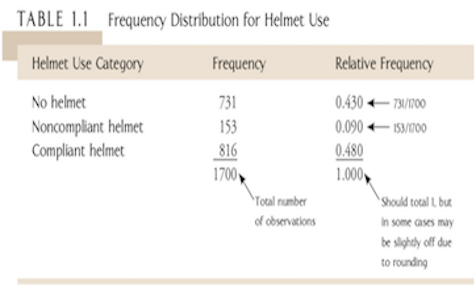
\includegraphics{fig1.1.png}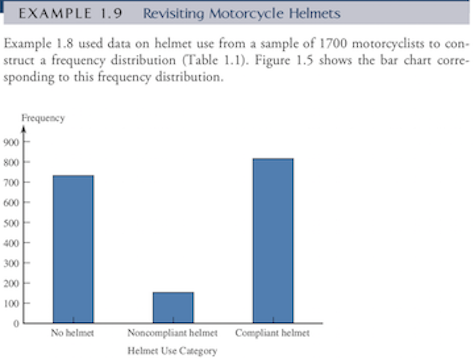
\includegraphics{fig1.2.png}

A \textbf{bar chart} is a graph of a frequency distribution of
categorical data. Each category in the frequency distribution is
represented by a bar or rectangle, and the picture is constructed in
such a way that the \emph{area} of each bar is proportional to the
corresponding frequency or relative frequency.

\end{frame}

\begin{frame}[fragile]{Bar plot: a basic example in R}

Suppose, we have a vector of maximum temperatures (in degree Celsius)
for seven days as follows

\begin{Shaded}
\begin{Highlighting}[]
\NormalTok{max.temp <-}\StringTok{ }\KeywordTok{c}\NormalTok{(}\DecValTok{22}\NormalTok{, }\DecValTok{27}\NormalTok{, }\DecValTok{26}\NormalTok{, }\DecValTok{24}\NormalTok{, }\DecValTok{23}\NormalTok{, }\DecValTok{26}\NormalTok{, }\DecValTok{28}\NormalTok{)}
\end{Highlighting}
\end{Shaded}

Now we can make a bar plot out of this data.

\begin{Shaded}
\begin{Highlighting}[]
\KeywordTok{barplot}\NormalTok{(max.temp)}
\end{Highlighting}
\end{Shaded}

\includegraphics{EDA_in_r_files/figure-beamer/unnamed-chunk-4-1.pdf}

\end{frame}

\begin{frame}{Data Visualisation: Comparative bar chart}

Bar charts can also be used to give a visual comparison of two or more
groups. This is accomplished by constructing two or more bar charts that
use the same set of horizontal and vertical axes, as illustrated in
Example 3.1.

\begin{figure}
\centering
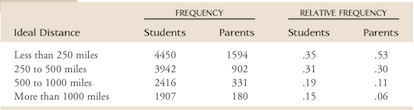
\includegraphics{fig1.3.png}
\caption{}
\end{figure}

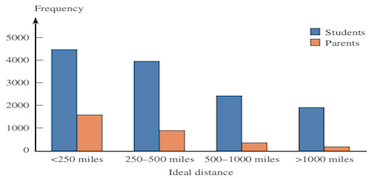
\includegraphics{fig1.4.png}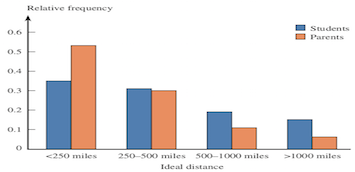
\includegraphics{fig1.5.png}

\end{frame}

\begin{frame}{Data Visualisation: Pie chart}

Categorical data with a relatively small number of possible categories.
Example: Scientists and Nonscientiest do not see Eye-to-Eye

Scientists and nonscientists were asked to indicate if they agreed or
disagreed with the following statement: ``When something is run by the
government, it is usually inefficient and wasteful.''

\begin{figure}
\centering
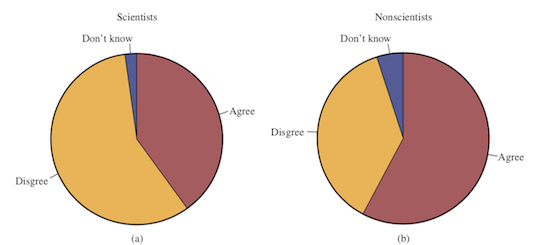
\includegraphics{fig1.6.png}
\caption{}
\end{figure}

\end{frame}

\begin{frame}[fragile]{Discrete Numerical Data Visualisation: Stemplots}

A stem-and-leaf display is an effective and compact way to summarize
univariate numerical data. Each number in the data set is broken into
two pieces, a stem and a leaf. The \textbf{stem} is the first part of
the number and consists of the beginning digit(s). The \textbf{leaf} is
the last part of the number and consists of the final digit(s).

\textbf{Example}: A noise metre was used to detect the noise level ( in
decibel ) during a concert in the Hong Kong stadium . The results are
recorded below.

\begin{Shaded}
\begin{Highlighting}[]
\NormalTok{d=}\KeywordTok{c}\NormalTok{(}\DecValTok{82}\NormalTok{,}\DecValTok{74}\NormalTok{,}\DecValTok{88}\NormalTok{,}\DecValTok{66}\NormalTok{,}\DecValTok{58}\NormalTok{,}\DecValTok{74}\NormalTok{,}\DecValTok{78}\NormalTok{,}\DecValTok{84}\NormalTok{,}\DecValTok{96}\NormalTok{,}\DecValTok{76}\NormalTok{,}\DecValTok{62}\NormalTok{,}\DecValTok{68}\NormalTok{,}\DecValTok{72}\NormalTok{,}\DecValTok{92}\NormalTok{,}\DecValTok{86}\NormalTok{,}\DecValTok{76}\NormalTok{,}\DecValTok{52}\NormalTok{,}
\DecValTok{76}\NormalTok{,}\DecValTok{82}\NormalTok{,}\DecValTok{78}\NormalTok{)}
\KeywordTok{stem}\NormalTok{(d)}
\end{Highlighting}
\end{Shaded}

\begin{verbatim}
## 
##   The decimal point is 1 digit(s) to the right of the |
## 
##   5 | 28
##   6 | 268
##   7 | 24466688
##   8 | 22468
##   9 | 26
\end{verbatim}

\end{frame}

\begin{frame}{Discrete Numerical Data Visualisation: Stemplots}

\textbf{Pros}:

\begin{itemize}
\item
  Easy to construct
\item
  Permit the viewer to reconstruct the data set
\item
  Easy to identify the order observations
\end{itemize}

\textbf{Cons}:

\begin{itemize}
\item
  Only suitable for describing small set of data
\item
  Little flexibility in the choice of stem
\item
  Does not convey a rapid reading of class frequency
\end{itemize}

\end{frame}

\begin{frame}{Data Visualisation: Frequency Distributions and Histogram}

As you have seen, a stemplot is not always an effective way to summarize
data; it is unwieldy when the data set contains a large number of
observations. Frequency distributions and histograms are displays that
work well for large data sets.

\end{frame}

\begin{frame}[fragile]{Frequency distribution: qualitative data}

Barplot is used to represent frequency distribution for
categorical/qualitative data

\begin{Shaded}
\begin{Highlighting}[]
\NormalTok{grade<-}\StringTok{ }\KeywordTok{c}\NormalTok{(}\StringTok{"A"}\NormalTok{,}\StringTok{"A"}\NormalTok{,}\StringTok{"B"}\NormalTok{,}\StringTok{"C"}\NormalTok{,}\StringTok{"D"}\NormalTok{,}\StringTok{"D"}\NormalTok{,}\StringTok{"A"}\NormalTok{,}\StringTok{"B"}\NormalTok{,}\StringTok{"C"}\NormalTok{,}\StringTok{"C"}\NormalTok{,}
          \StringTok{"B"}\NormalTok{,}\StringTok{"A"}\NormalTok{,}\StringTok{"A"}\NormalTok{,}\StringTok{"B"}\NormalTok{,}\StringTok{"B"}\NormalTok{,}\StringTok{"C"}\NormalTok{,}\StringTok{"A"}\NormalTok{,}\StringTok{"A"}\NormalTok{,}\StringTok{"A"}\NormalTok{,}\StringTok{"C"}\NormalTok{)}
\KeywordTok{library}\NormalTok{(plyr)}
\NormalTok{y<-}\KeywordTok{count}\NormalTok{(grade)}
\KeywordTok{barplot}\NormalTok{(y}\OperatorTok{$}\NormalTok{freq,}\DataTypeTok{names.arg=}\NormalTok{y}\OperatorTok{$}\NormalTok{x,}\DataTypeTok{main=}\StringTok{"Frequency Table of Grades"}\NormalTok{,}\DataTypeTok{col=}\KeywordTok{c}\NormalTok{(}\StringTok{"red"}\NormalTok{,}\StringTok{"blue"}\NormalTok{,}\StringTok{"green"}\NormalTok{,}\StringTok{"yellow"}\NormalTok{))}
\end{Highlighting}
\end{Shaded}

\includegraphics{EDA_in_r_files/figure-beamer/unnamed-chunk-6-1.pdf}

\end{frame}

\begin{frame}[fragile]{Relative frequency}

\begin{Shaded}
\begin{Highlighting}[]
\NormalTok{n<-}\KeywordTok{sum}\NormalTok{(y}\OperatorTok{$}\NormalTok{freq)}
\NormalTok{rf<-}\StringTok{ }\NormalTok{y}\OperatorTok{$}\NormalTok{freq}\OperatorTok{/}\NormalTok{n}
\KeywordTok{barplot}\NormalTok{(rf,}\DataTypeTok{names.arg=}\NormalTok{y}\OperatorTok{$}\NormalTok{x,}\DataTypeTok{main=}\StringTok{"Frequency Table of Grades"}\NormalTok{,}\DataTypeTok{col=}\KeywordTok{c}\NormalTok{(}\StringTok{"red"}\NormalTok{,}\StringTok{"blue"}\NormalTok{,}\StringTok{"green"}\NormalTok{,}\StringTok{"yellow"}\NormalTok{))}
\end{Highlighting}
\end{Shaded}

\includegraphics{EDA_in_r_files/figure-beamer/unnamed-chunk-7-1.pdf}

\end{frame}

\begin{frame}{Frequency distribution for quantitative data}

A frequency distribution is a tabular presentation of statistical data
that aids the analysis of large data sets. Frequency distribution
summarize statistical data by assigning it to specified groups, or
intervals.

\textbf{Procedure}

\begin{itemize}
\item
  Step 1: Define the intervals.
\item
  Step 2: Tally the observations.
\item
  Step 3: Count the observations.
\end{itemize}

\end{frame}

\begin{frame}{Example}

\begin{figure}
\centering
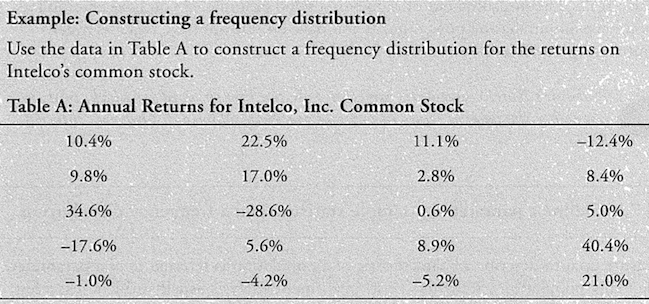
\includegraphics{fig1.7.png}
\caption{Annual Returns for ABC Common stock}
\end{figure}

\end{frame}

\begin{frame}{Data Visualisation: Histogram}

\includegraphics{EDA_in_r_files/figure-beamer/unnamed-chunk-8-1.pdf}

\end{frame}

\begin{frame}[fragile]{Data Visualisation/Spread measure: Boxplot}

\begin{Shaded}
\begin{Highlighting}[]
\KeywordTok{boxplot}\NormalTok{(data}\OperatorTok{$}\NormalTok{bill,}\DataTypeTok{horizontal=}\OtherTok{TRUE}\NormalTok{)}
\end{Highlighting}
\end{Shaded}

\includegraphics{EDA_in_r_files/figure-beamer/unnamed-chunk-9-1.pdf}

\end{frame}

\begin{frame}{Data Visualisation: Scatterplot}

See lecture 2.

\end{frame}

\begin{frame}{Numerical Descriptions of Data}

\begin{itemize}
\item
  A measure used to describe a characteristic of a population is
  referred to as a \textbf{parameter}. Examples: mean and standard
  deviation.
\item
  Likewise, a \textbf{sample statistic} is used to measure a
  characteristic of a sample.
\item
  In order to distinguish between parameters and statistics, different
  notations are used:

  \begin{itemize}
  \item
    Greek letter for parameter (e.g. \(\mu\) and \(\sigma\))
  \item
    Roman letter for statistic (e.g. \(\bar{x}\) and \(s\))
  \end{itemize}
\item
  Parameter are fixed (\emph{typically unknown}) and statistics are
  random (\emph{observed from our sample})
\end{itemize}

\end{frame}

\begin{frame}{Symmetry}

\begin{itemize}
\item
  The symmetry of a distribution is measured by calculating the skewness
  of the distribution.

  \begin{itemize}
  \item
    Negative skewness: \textbf{left skewed} distribution.
  \item
    Positive skewness: \textbf{right skewed} distribution.
  \item
    Skewness close to 0, reasonably \textbf{symmetric} distribution.
  \end{itemize}
\item
  In general, we will only state that a distribution is skewed if the
  skew is strong and obvious. 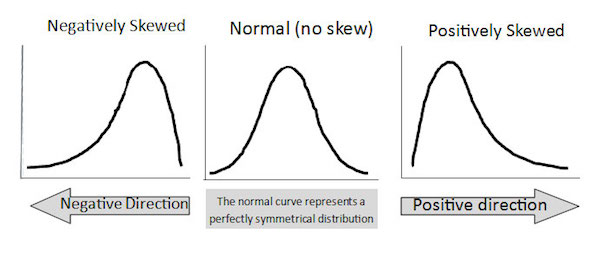
\includegraphics{measure-of-skewness.jpg} 
\end{itemize}

\end{frame}

\begin{frame}{Measures of Central Tendency}

\begin{itemize}
\item
  One important feature of the data we collect is the location of the
  data, that is, what are typical value of my observations?
\item
  One way to describe the location of the data is to calculate a measure
  of central tendency. That is, where is the middle of the data?
\item
  Three common measures of central tendency.

  \begin{itemize}
  \item
    Mean : average
  \item
    Median: middle, depends on data being ordered.
  \item
    Mode: most frequent observations?
  \end{itemize}
\end{itemize}

\end{frame}

\begin{frame}{Measures of Central Tendency: Mean}

\begin{itemize}
\item
  Sample mean

  \begin{itemize}
  \tightlist
  \item
    With sample size \(n\)
    \[\bar{X}=\frac{\sum^n_{i=1}x_i}{n}=\frac{x_1+x_2+\cdots+x_n}{n}\]
  \end{itemize}
\item
  Polulation mean

  \begin{itemize}
  \tightlist
  \item
    With population size \(N\)
    \[\mu=\frac{\sum^N_{i=1}x_i}{n}=\frac{x_1+x_2+\cdots+x_N}{N}\]
  \end{itemize}
\end{itemize}

\end{frame}

\begin{frame}{Measures of Central Tendency: Mean}

\begin{itemize}
\item
  Issues with using the mean:

  \begin{itemize}
  \item
    Can be sensitive to skewness.
  \item
    The mean can be very sensitive to a few extreme values (Outliers).
  \end{itemize}
\item
  So we use the mean when the distribution is not strongly skewed, and
  has no outliers.
\end{itemize}

\end{frame}

\begin{frame}{Measures of Central Tendency: Median}

The median is the middle data point, after the data is ordered from
smallest to largest.

\begin{itemize}
\item
  If \(n\) is odd, then the median is the unique middle point as
  \(x_{\frac{n+1}{2}}\).
\item
  If \(n\) is even, the median is the average of 2 middle values. That
  is \(\frac{x_{n/2}+x_{n/2+1}}{2}\)
\end{itemize}

\end{frame}

\begin{frame}{Measure of Central Tendency: Mode}

\begin{itemize}
\item
  The mode is the value that occurs most often.

  \begin{itemize}
  \item
    The mode is not affected by extreme values.
  \item
    There may be more than one mode.
  \item
    The mode may not exist at all.
  \item
    Used for either numerical or categorical data
  \end{itemize}
\end{itemize}

\end{frame}

\begin{frame}[fragile]{Pizza delivery dataset}

The pizza delivery dataset refers to an Italian restaurant which offers
home delivery of pizza.

\begin{Shaded}
\begin{Highlighting}[]
\CommentTok{#Read in data}
\NormalTok{data=}\KeywordTok{read.csv}\NormalTok{(}\StringTok{"DATA//pizza_delivery.csv"}\NormalTok{,}\DataTypeTok{header=}\NormalTok{T)}
\CommentTok{#Names of variables}
\KeywordTok{names}\NormalTok{(data)}
\end{Highlighting}
\end{Shaded}

\begin{verbatim}
##  [1] "day"               "date"              "time"             
##  [4] "operator"          "branch"            "driver"           
##  [7] "temperature"       "bill"              "pizzas"           
## [10] "free_wine"         "got_wine"          "discount_customer"
\end{verbatim}

\end{frame}

\begin{frame}[fragile]{Pizza delivery dataset}

\begin{itemize}
\tightlist
\item
  Structure of Data
\end{itemize}

\begin{Shaded}
\begin{Highlighting}[]
\KeywordTok{str}\NormalTok{(data)}
\end{Highlighting}
\end{Shaded}

\begin{verbatim}
## 'data.frame':    1266 obs. of  12 variables:
##  $ day              : Factor w/ 7 levels "Friday","Monday",..: 5 5 5 5 5 5 5 5 5 5 ...
##  $ date             : Factor w/ 31 levels "01-May-14","02-May-14",..: 1 1 1 1 1 1 1 1 1 1 ...
##  $ time             : num  35.1 25.2 45.6 29.4 30 ...
##  $ operator         : Factor w/ 2 levels "Laura","Melissa": 1 2 2 2 2 2 1 2 1 2 ...
##  $ branch           : Factor w/ 3 levels "Centre","East",..: 2 2 3 2 3 1 3 3 1 1 ...
##  $ driver           : Factor w/ 5 levels "Bruno","Domenico",..: 1 5 5 5 5 1 1 4 4 1 ...
##  $ temperature      : num  68.3 71 53.4 70.3 71.5 ...
##  $ bill             : num  58.4 26.4 58.1 35.2 38.4 61.8 57.9 35.8 36.6 44.8 ...
##  $ pizzas           : int  4 2 3 3 2 4 3 2 2 5 ...
##  $ free_wine        : int  0 0 1 0 0 1 1 0 0 0 ...
##  $ got_wine         : int  0 0 0 0 0 1 1 0 0 0 ...
##  $ discount_customer: int  1 0 0 0 0 0 0 0 0 0 ...
\end{verbatim}

\end{frame}

\begin{frame}[fragile]{Numerical summaries: Central tendency}

We can find mean and median by hand. However, here our sample size is
1266. It is tedious to compute mean over these many observations.
Fortunately we have R to perform this task.

\begin{Shaded}
\begin{Highlighting}[]
\KeywordTok{mean}\NormalTok{(data}\OperatorTok{$}\NormalTok{bill)}
\end{Highlighting}
\end{Shaded}

\begin{verbatim}
## [1] 42.75592
\end{verbatim}

\begin{Shaded}
\begin{Highlighting}[]
\KeywordTok{median}\NormalTok{(data}\OperatorTok{$}\NormalTok{bill)}
\end{Highlighting}
\end{Shaded}

\begin{verbatim}
## [1] 42.9
\end{verbatim}

\begin{itemize}
\item
  How did you find median?

  \begin{itemize}
  \tightlist
  \item
    As the size of the data is 1266 (even), the median is found between
    the 633rd and 634th bill, or \(\frac{42.9+42.9}{2}=42.9\).
  \end{itemize}
\item
  To find mode, sadly there is no R in-built function to use. Hence we
  have to create our own.
\end{itemize}

\begin{Shaded}
\begin{Highlighting}[]
\NormalTok{x<-data}\OperatorTok{$}\NormalTok{bill}
\NormalTok{y=}\KeywordTok{names}\NormalTok{(}\KeywordTok{table}\NormalTok{(x))[}\KeywordTok{table}\NormalTok{(x)}\OperatorTok{==}\KeywordTok{max}\NormalTok{(}\KeywordTok{table}\NormalTok{(x))]}
\NormalTok{y}
\end{Highlighting}
\end{Shaded}

\begin{verbatim}
## [1] "36.2"
\end{verbatim}

\end{frame}

\begin{frame}[fragile]{Mean, Median and Mode on the histogram}

\begin{Shaded}
\begin{Highlighting}[]
\KeywordTok{hist}\NormalTok{(data}\OperatorTok{$}\NormalTok{bill)}
\KeywordTok{abline}\NormalTok{(}\DataTypeTok{v=}\KeywordTok{mean}\NormalTok{(data}\OperatorTok{$}\NormalTok{bill),}\DataTypeTok{col=}\StringTok{"green"}\NormalTok{)}
\KeywordTok{abline}\NormalTok{(}\DataTypeTok{v=}\KeywordTok{median}\NormalTok{(data}\OperatorTok{$}\NormalTok{bill),}\DataTypeTok{col=}\StringTok{"purple"}\NormalTok{)}
\KeywordTok{abline}\NormalTok{(}\DataTypeTok{v=}\NormalTok{y,}\DataTypeTok{col=}\StringTok{"pink"}\NormalTok{)}
\end{Highlighting}
\end{Shaded}

\includegraphics{EDA_in_r_files/figure-beamer/unnamed-chunk-14-1.pdf}

\end{frame}

\begin{frame}[fragile]{Mean, median and Mode on the boxplot}

\begin{itemize}
\tightlist
\item
  The median is the centre line on the boxplot.
\end{itemize}

\begin{Shaded}
\begin{Highlighting}[]
\KeywordTok{boxplot}\NormalTok{(data}\OperatorTok{$}\NormalTok{bill)}
\KeywordTok{abline}\NormalTok{(}\DataTypeTok{h=}\KeywordTok{mean}\NormalTok{(data}\OperatorTok{$}\NormalTok{bill),}\DataTypeTok{col=}\StringTok{"green"}\NormalTok{)}
\KeywordTok{abline}\NormalTok{(}\DataTypeTok{h=}\KeywordTok{median}\NormalTok{(data}\OperatorTok{$}\NormalTok{bill),}\DataTypeTok{col=}\StringTok{"purple"}\NormalTok{)}
\KeywordTok{abline}\NormalTok{(}\DataTypeTok{h=}\KeywordTok{mode}\NormalTok{(data}\OperatorTok{$}\NormalTok{bill),}\DataTypeTok{col=}\StringTok{"pink"}\NormalTok{)}
\end{Highlighting}
\end{Shaded}

\begin{verbatim}
## Warning in int_abline(a = a, b = b, h = h, v = v, untf = untf, ...): NAs
## introduced by coercion
\end{verbatim}

\includegraphics{EDA_in_r_files/figure-beamer/unnamed-chunk-15-1.pdf}

As you see, both histogram and boxplot suggest that the mean and median
of total bills from pizza delivery is about the same. In other words,
our data is fairly symmetric. Note, this is not necessarily the case in
practice. Very often, the two statistics differ greatly from each other
due to outliers. In general, the median is more robust and a good
summary for skewed data as it is NOT affected by outliers.

\end{frame}

\begin{frame}{Measure of Spread}

\begin{itemize}
\item
  Range
\item
  Variance
\item
  Standard Deviation
\item
  Quartile, IQR
\end{itemize}

\end{frame}

\begin{frame}{Measure of Spread: Range}

\begin{itemize}
\tightlist
\item
  Difference between the \textbf{largest} and the \textbf{smallest}
  observations:
\end{itemize}

\[\text{Range}=X_{\text{Largest}}-X_{\text{Smallest}}\]

\end{frame}

\begin{frame}{Measures of Spread: Variance}

\begin{itemize}
\item
  Average (squared) distance of an observation from the mean.
\item
  Variances of independent measurements \textbf{can be added together}
  (standard deviation cannot be added).

  \begin{itemize}
  \tightlist
  \item
    Sample Variance:
    \[s^2=\frac{\sum^n_{i=1}(X_i-\overline{X})^2}{n-1}\]
  \item
    \[\sigma^2=\frac{\sum^N_{i=1}(x_i-\mu)^2}{N}\] Caution: the sample
    variance has a denominator of \(n-1\), butthe population variance
    has a denominator of \(N\).
  \end{itemize}
\end{itemize}

\end{frame}

\begin{frame}{Measures of Spread: Standard Deviation}

\begin{itemize}
\item
  The positive square root of the variance.
\item
  It is easier to interpret as it has the \textbf{same units} as the
  data itself.

  \begin{itemize}
  \item
    Sample Standard Deviation:
    \[ s=\sqrt{\frac{\sum^n_{i=1}(X_i-\overline{X})^2}{n-1}} \]
  \item
    Population Standard Deviation:
    \[ s=\sqrt{\frac{\sum^n_{i=1}(x_i-\mu)^2}{N}} \]
  \end{itemize}
\end{itemize}

\end{frame}

\begin{frame}{Measures of Spread: Quartiles (IQR)}

\begin{itemize}
\item
  The quartiles are a set of 3 values (Q1, Q2, Q3) that roughly split
  the data into quarters
\item
  Q1 is the 25th percentile point
\item
  Q2 is the median
\item
  Q3 is the 75th percentile point
\item
  IQR is equal to Q3-Q1 which represent the length of middle 50\% of the
  data set.

  \begin{itemize}
  \tightlist
  \item
    Just like the median, the IQR is \textbf{robust}, so it is suitable
    as a summary of spread for skewed data
  \end{itemize}
\end{itemize}

\end{frame}

\begin{frame}{The Five Number Summary}

\begin{itemize}
\tightlist
\item
  One neat way to summarise the data is the 5 number summary, which is
  drawn by the boxplot. \includegraphics{boxplot.gif}
\end{itemize}

\end{frame}

\begin{frame}{Comparing the mean and the median}

The difference between the mean and the median can be an indication of
the \textbf{shape} of the data.

\begin{itemize}
\item
  For symmetric data, we expect the mean and median to be the same
\item
  For left skewed data, we expect the mean to be smaller than the median
\item
  For right skewed data, we expect the mean to be larger than the median
\end{itemize}

\begin{figure}
\centering
\includegraphics{mean\&median.png}
\caption{}
\end{figure}

\end{frame}

\begin{frame}[fragile]{HW exercise}

\begin{itemize}
\tightlist
\item
  Given a data set (9,10,10.5,12,14,17), find mean, variance and
  standard deviation by hand.
\end{itemize}

In R, define

\begin{Shaded}
\begin{Highlighting}[]
\NormalTok{x<-}\StringTok{ }\KeywordTok{c}\NormalTok{(}\DecValTok{9}\NormalTok{,}\DecValTok{10}\NormalTok{,}\FloatTok{10.5}\NormalTok{,}\DecValTok{12}\NormalTok{,}\DecValTok{14}\NormalTok{,}\DecValTok{17}\NormalTok{)}
\NormalTok{miu<-}\StringTok{ }\KeywordTok{mean}\NormalTok{(x)}
\NormalTok{variance<-}\StringTok{ }\KeywordTok{var}\NormalTok{(x)}
\NormalTok{sdtv<-}\StringTok{ }\KeywordTok{sqrt}\NormalTok{(variance)}
\NormalTok{miu}
\end{Highlighting}
\end{Shaded}

\begin{verbatim}
## [1] 12.08333
\end{verbatim}

\begin{Shaded}
\begin{Highlighting}[]
\NormalTok{variance}
\end{Highlighting}
\end{Shaded}

\begin{verbatim}
## [1] 8.841667
\end{verbatim}

\begin{Shaded}
\begin{Highlighting}[]
\NormalTok{sdtv}
\end{Highlighting}
\end{Shaded}

\begin{verbatim}
## [1] 2.973494
\end{verbatim}

\end{frame}

\begin{frame}{IQR on the boxplot}

\begin{itemize}
\item
  As discussed earlier, the IQR is the length of the box. It represents
  the span of the middle 50\% of the data.
\item
  The \textbf{lower} and \textbf{upper thresholds} are a distance of 1.5
  from the quartiles (by convention)
\end{itemize}

\[ \text{LT}=Q1-1.5\, \text{IQ}R \] and
\[ \text{UT}=Q3+1.5\, \text{IQ}R \]

\begin{itemize}
\tightlist
\item
  Data outside these thresholds is considered an outlier.
\end{itemize}

\end{frame}

\begin{frame}[fragile]{Back to Pizza delivery dataset}

\begin{Shaded}
\begin{Highlighting}[]
\KeywordTok{boxplot}\NormalTok{(data}\OperatorTok{$}\NormalTok{bill)}
\NormalTok{iqr=}\KeywordTok{quantile}\NormalTok{(data}\OperatorTok{$}\NormalTok{bill)[}\DecValTok{4}\NormalTok{]}\OperatorTok{-}\KeywordTok{quantile}\NormalTok{(data}\OperatorTok{$}\NormalTok{bill)[}\DecValTok{2}\NormalTok{]}
\KeywordTok{abline}\NormalTok{(}\DataTypeTok{h=}\KeywordTok{median}\NormalTok{(data}\OperatorTok{$}\NormalTok{bill),}\DataTypeTok{col=}\StringTok{"pink"}\NormalTok{)}
\KeywordTok{abline}\NormalTok{(}\DataTypeTok{h=}\KeywordTok{quantile}\NormalTok{(data}\OperatorTok{$}\NormalTok{bill)[}\DecValTok{2}\NormalTok{]}\OperatorTok{-}\FloatTok{1.5}\OperatorTok{*}\NormalTok{iqr,}\DataTypeTok{col=}\StringTok{"purple"}\NormalTok{)}
\KeywordTok{abline}\NormalTok{(}\DataTypeTok{h=}\KeywordTok{quantile}\NormalTok{(data}\OperatorTok{$}\NormalTok{bill)[}\DecValTok{2}\NormalTok{]}\OperatorTok{+}\FloatTok{1.5}\OperatorTok{*}\NormalTok{iqr,}\DataTypeTok{col=}\StringTok{"purple"}\NormalTok{)}
\end{Highlighting}
\end{Shaded}

\includegraphics{EDA_in_r_files/figure-beamer/unnamed-chunk-17-1.pdf}

Note, there exists quite a few outliers out of the 1266 pizza bills!

\end{frame}

\end{document}
